\section{Optimización de Hiperparámetros}

Sea $f: X \rightarrow \mathbb{R}$ una función que devuelve el máximo error de validación de un modelo entrenado a partir de una combinación de hiperparámetros $\textbf{x} \in X$, se desea encontrar $\hat{\textbf{x}}$:

\[
\hat{\textbf{x}} = arg \min_{\textbf{x} \in X} f(\textbf{x})
\]

Es decir, se busca encontrar la combinación óptima de hiperparámetros dentro de un dominio $X$ para obtener el mínimo error de representación en un dado conjunto de validación.En el caso de la construcción de una base \textit{hp-greedy} óptima: 

\[
\textbf{x} = (n_{max}, l_{max}, \varepsilon, \hat{\Lambda}_0)
\]

El hiperparámetro de mayor interés es sin duda la $semilla$, pues a primera vista no hay una forma obvia de elegir su valor óptimo. Además una semilla óptima para una combinación de $(n_{max_1}, l_{max_1})$ no lo será necesariamente para otra combinación $(n_{max_2}, l_{max_2})$.

También se observó que en ciertas situaciones un valor muy elevado de $l_{max}$ o muy pequeño de la $tolerancia$ $greedy$ pueden conducir a un modelo \textit{sobreajustado}. Por esto es de interés realizar una optimización que involucre a la totalidad de los hiperparámetros dentro del dominio $X$. 


El problema al momento de realizar esta optimización es que la función $f$ no es una función analítica, sino es que es el resultado de entrenar el modelo y evaluar el error de representación con un conjunto de validación, lo que la hace costosa de evaluar (computacionalmente hablando). Esta sección se centrará en la \textbf{optimización Bayesiana} \cite{7352306, https://doi.org/10.48550/arxiv.1012.2599}, un método que intenta reducir al mínimo el número de evaluaciones de $f$ para encontrar $\hat{\textbf{x}}$ y se puede colocar dentro de una categoría llamada optimización secuencial basada en modelos, o \textbf{SMBO}\cite{dewancker2015bayesian,NIPS2011_86e8f7ab} (\textit{Secuential Model-Based Optimization}).


Además existen dos métodos muy utilizados que no utilizan modelos, los cuales son la busqueda exaustiva (o \textit{grid search}) y la búsqueda aleatoria. Antes de hablar de la optimización Bayesiana se introducirá brevemente dl método de la búsqueda exhaustiva para luego realizar una comparación entre ambos métodos en un problema de optimización relativamente sencillo.


\subsection{Búsqueda Exhaustiva}

 
 
 
 La búsqueda exhaustiva o \textit{grid search} consiste en probar todas las combinaciones posibles dentro de un espacio de hiperparámetros para seleccionar la solución óptima. Es decir que si se quiere buscar la combinación óptima de $(n_{max}, l_{max})$ para un rango de valores $n_{max} \in N,$ $l_{max} \in L$ se deberán probar todas las combinaciones posibles del producto cartesiano $N \times L = \{(n_{max}, l_{max}) | n_{max} \in N, l_{max} \in L\}$. 
 
La ventaja de este método está en que el resultado óptimo está garantizado, pues se pueden comparar todos los resultados entre sí y elegir el mejor. El problema es que, como se mencionó, la función $f$ es costosa de evaluar, y por otro lado el número de combinaciones posibles escala exponencialmente con cada hiperparámetro extra a optimizar (además se debe tener en cuenta que la semilla $\hat{\Lambda}_0$ tendrá generalmente más de una dimension).

Por estas razones la búsqueda exhaustiva no será un método viable en la mayoría de los casos que son de interés para este trabajo. Sin embargo se puede poner a prueba con casos simplificados para luego comparar los resultados con otros métodos más eficaces.

\begin{figure}[h!]
\centering
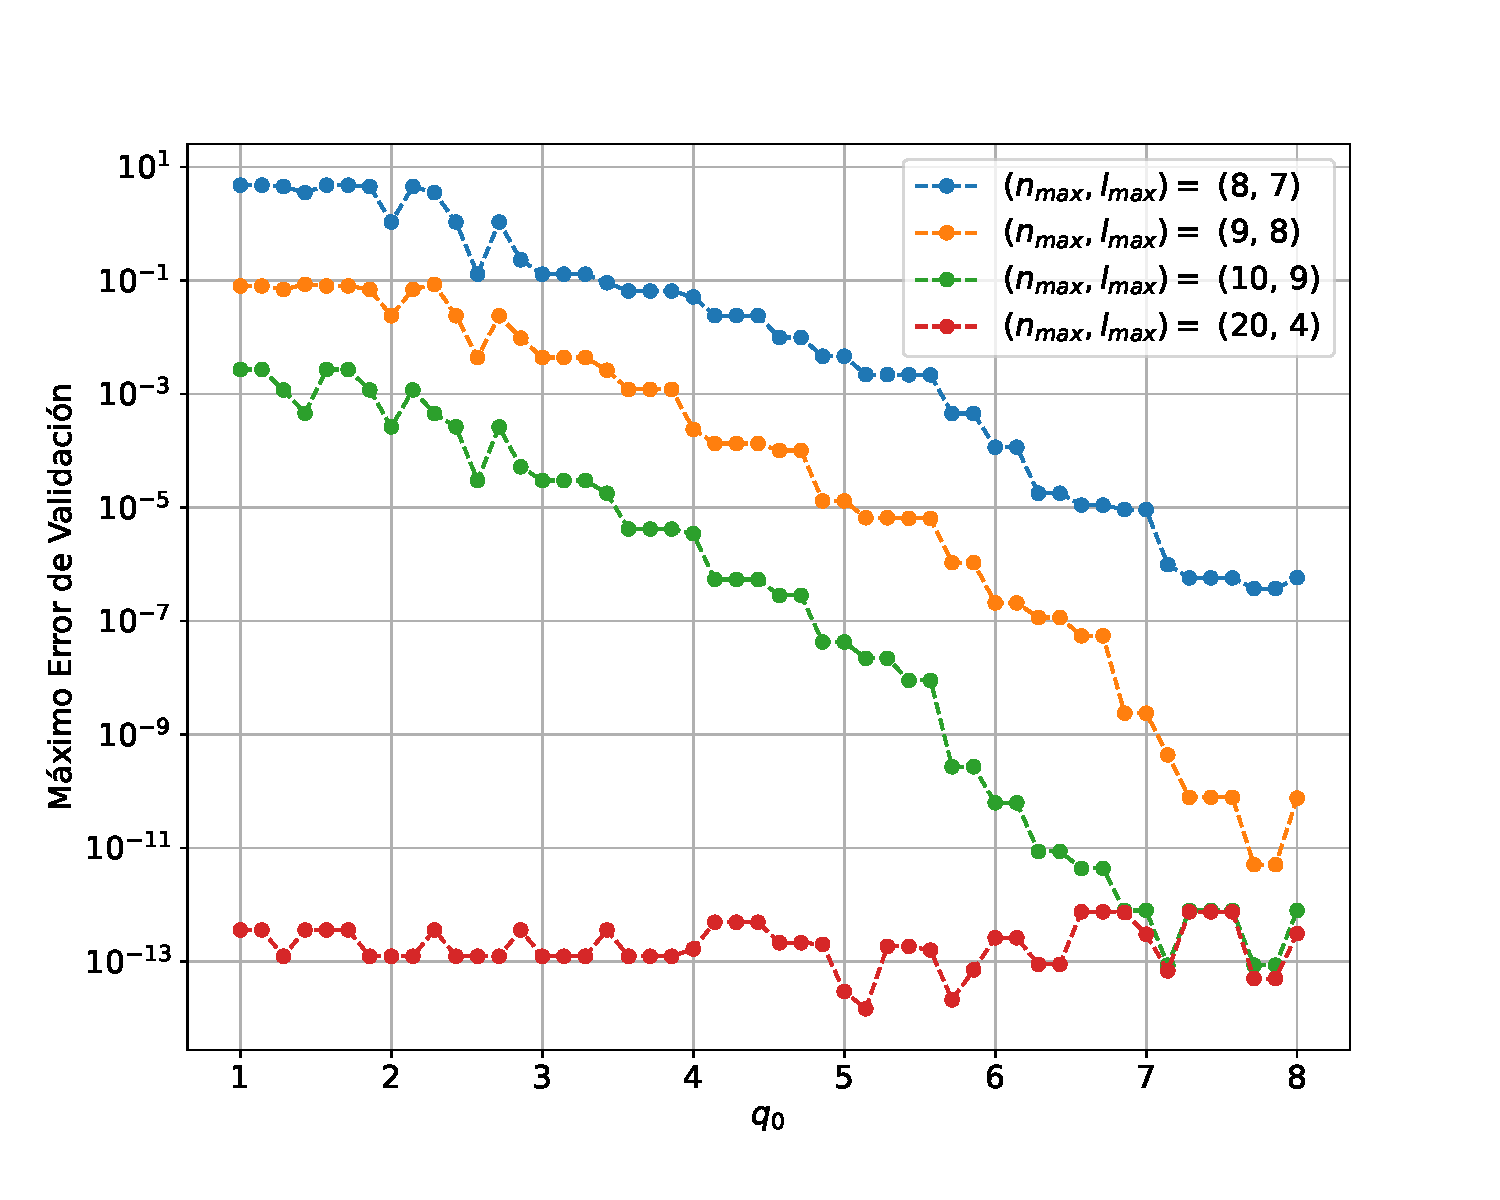
\includegraphics[width=.8\columnwidth, trim={1.1cm, 1cm, 1cm, 1.2cm}]{grid_seeds_0.pdf}
\caption{Variación de la semilla $q_0$ para distintas combinaciones de $(n_{max}, l_{max})$}
\label{fig:grid_seed_0}
\end{figure}

Por ejemplo, para un conjunto de entrenamiento con cincuenta ondas equidistantes en el espacio del parámetro unidimensional $q: 1 < q < 8$, se quiere optimizar el error de representación para un conjunto de validación con mil ondas. Los hiperparámetros a optimizar son $\textbf{x} = (n_{max}, l_{max}, \hat{\Lambda}_0)$, dejando $\varepsilon$ fijo en $1\times 10^{-12}$ para simplificar la búsqueda, que se realiza en los siguientes intervalos:

\begin{align*}
n_{max} &\in [5, 20],\\
l_{max} &\in [1, 10],\\
\hat{\Lambda}_0 &\in \{q_0 \ | \ q_0 = 1 + i \Delta q, \ i\in \mathbb{N} : 0 \le i \le 49, \ \Delta q = 7/49 \}.
\end{align*}

Son 16 valores de $n_{max}$, 10 valores de $l_{max}$ y 50 para $q_0$ ($\hat{\Lambda}_0 = q_0$). Lo que hace un total de 8000 combinaciones posibles.



\begin{figure}[h!]
\centering
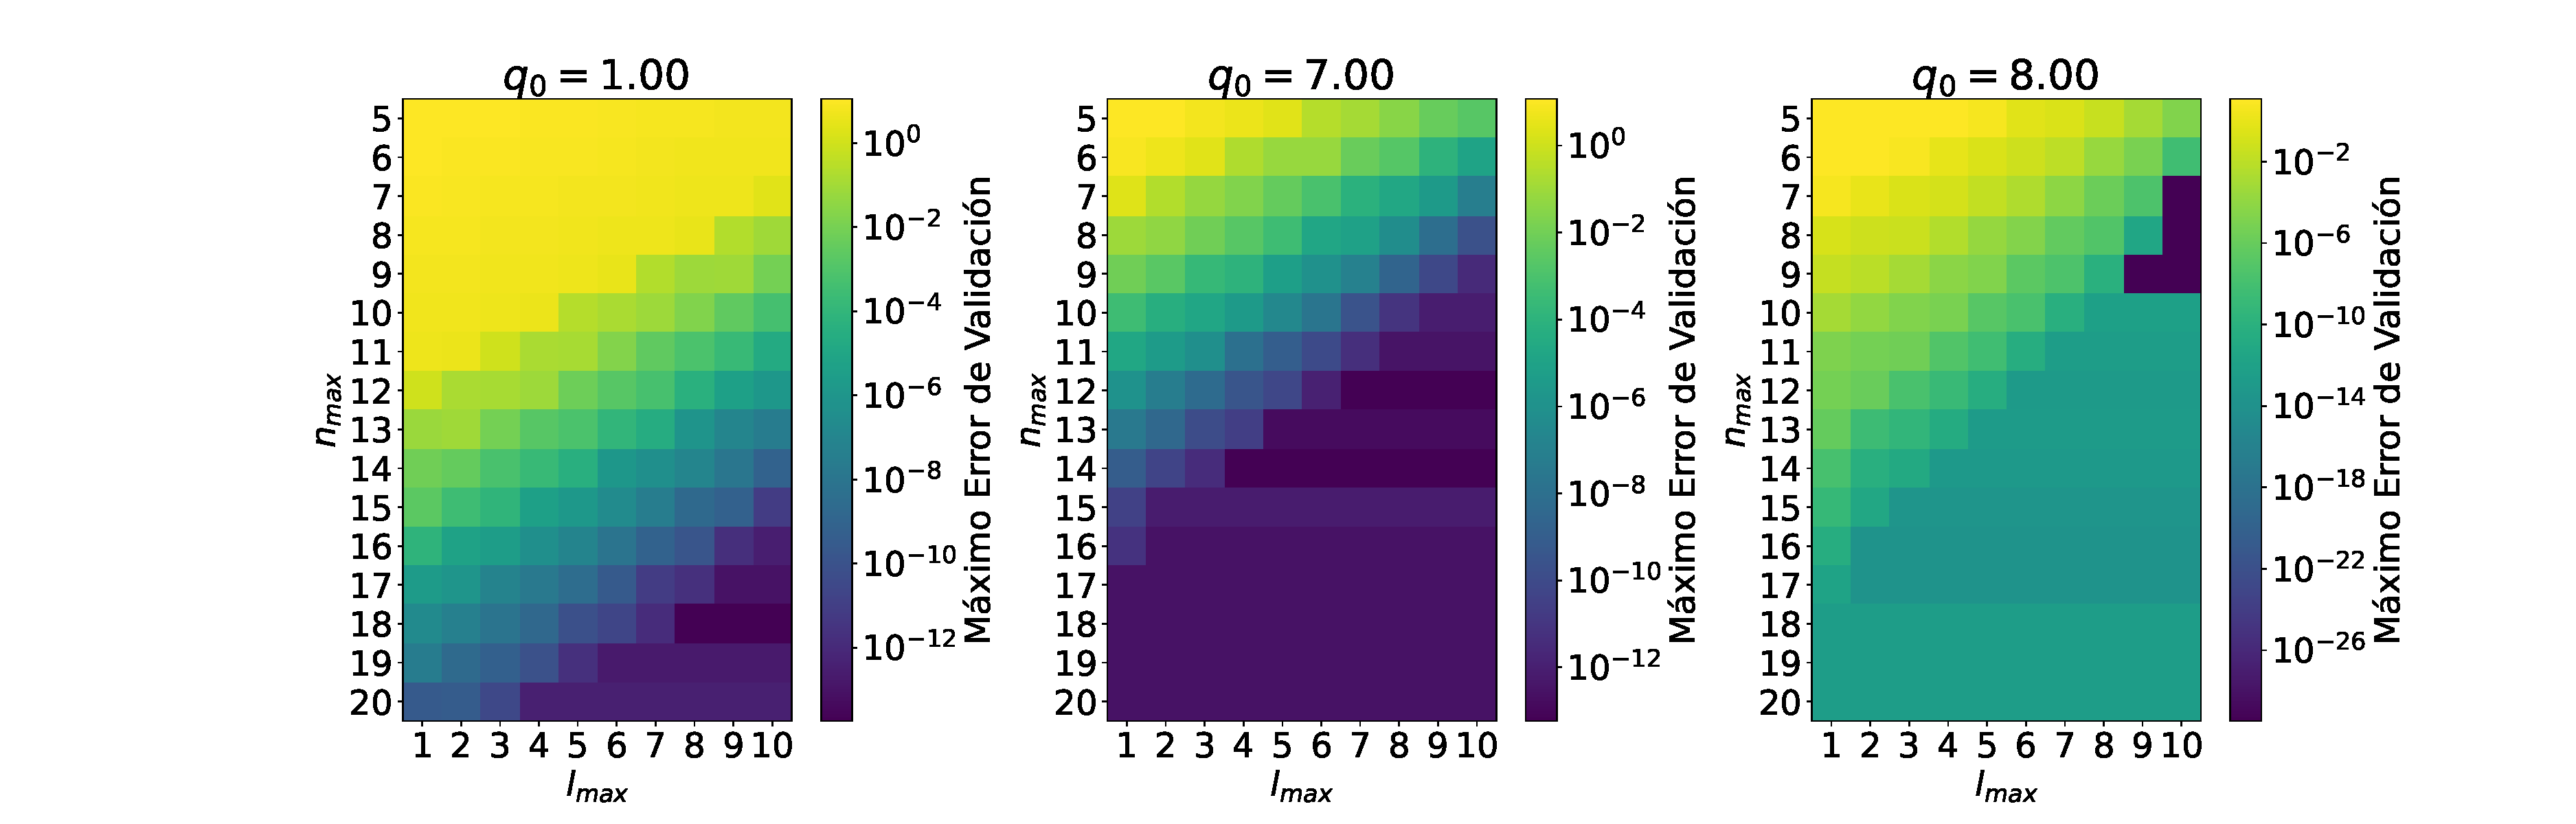
\includegraphics[width=1.05\columnwidth, trim={8cm, 1cm, 5cm, 1.1cm}]{grid_3_seeds.pdf}
\caption{Máximo error de validación en función de $n_{max}$ y $l_{max}$ para tres diferentes semillas $q_0$. }
\label{fig:grid_3_seeds}
\end{figure}

Si bien no se puede graficar el error en función de los tres hiperparámetros a la vez, se puede obtener bastante información al dejar fijo uno o dos hiperparámetros. Por ejemplo en la figura \ref{fig:grid_seed_0} se ven los resultados de variar únicamente la semilla para diferentes combinaciones de $n_{max}$ y $l_{max}$. Se observa que en este conjunto de datos la semilla suele ser óptima a valores cercanos a $q_0 = 8$, pero a la vez al aumentar el $n_{max}$ la influencia de la semilla es menor; con $(n_{max}, l_{max})=(20, 4)$ hay una diferencia de un orden de magnitud entre la mejor y la peor semilla, mientras que con $(n_{max}, l_{max})=(10, 9)$, por ejemplo, hay una diferencia de diez ordenes de magnitud.

Luego, en la figura \ref{fig:grid_3_seeds} se observa el error de validación en función de las combinaciones posibles de  $n_{max}$ y $l_{max}$ para tres diferentes semillas. A la derecha, con $q_0=8$ se observa el mejor error de representación obtenido en la búsqueda exhaustiva, con un valor de $4\times10^{-30}$ (el cual se obtuvo para 16 combinaciones de hiperparámetros), casi 15 ordenes de magnitud menor que el siguiente mejor error.


\subsection{Optimización Secuencial Basada en Modelos (SMBO)}


La optimización secuencial basada en modelos es un formalismo que es útil para explicar de manera general el funcionamiento de la optimización bayesiana.

La ventaja de este método es que cada evaluación de la función $f$ se decide en base al conjunto $D$ de observaciones realizadas previamente. Esto se logra entrenando un modelo sustituto $\mathcal{M}$ en base al conjunto $D$, y luego utilizando una función $S$ llamada función de \textit{adquisición}, que decidirá el mejor punto a evaluar en la función real.

Se parte de un conjunto $D$ generado a partir de un muestreo de observaciones de la función $f$ de la forma $(\textbf{x}_j, f(\textbf{x}_j))$, a partir del cual se ajusta el modelo sustituto $\mathcal{M}$. Luego, maximizando la función de adquisición $S$ se elije el siguiente conjunto de hiperparámetros $\textbf{x}_i$ para evaluar la función $f$ y se agrega el par $(\textbf{x}_i, f(\textbf{x}_i))$ al conjunto de observaciones $D$. Una vez hecho esto se vuelve a ajustar el modelo $\mathcal{M}$ y se repite el proceso, que está explicado en forma de pseudocódigo en el algoritmo \ref{alg:SMBO}.


\begin{algorithm}
\caption{\texttt{SMBO}}
\label{alg:SMBO}
\begin{algorithmic}[1]
\Require $f, X, S,\mathcal{M}$
\State $D =$ InicializarMuestras$(f, X)$
\vspace{1mm}
\For{$i = 1, 2, ...$}
	\State $\mathcal{M} =$ AjustarModelo$(D)$
	\State $\textbf{x}_{i} = arg \max_{\textbf{x}\in X} \mathcal{S}(\textbf{x}, \mathcal{M})$ .
	\State $y_i = f(\textbf{x}_i)$	\Comment{Paso costoso}
	\State $D = D \cup \{(\textbf{x}_i, y_i)\}$
\EndFor
\vspace{3mm}

\end{algorithmic}
\end{algorithm}




\subsection{Optimización Bayesiana}

Lo que caracteriza a la optimización bayesiana dentro del formalismo de la optimización secuencial basada en modelos, es justamente la creación del modelo.
En la optimización bayesiana se construye un modelo estadístico, donde se representa con  $P(y|\textbf{x})$ la predicción del modelo, siendo $y$ el resultado de una evaluación $f(\textbf{x})$. El nombre del método se debe a que para la construcción del modelo se utiliza el teorema de Bayes:
  
 \[
 P(y|\textbf{x}) = \frac{P(\textbf{x}|y) \ P(y)}{P(\textbf{x})}
 \]
 
 En la terminología bayesiana, se conoce a $P(y|\textbf{x})$ como probabilidad a posteriorí o \textit{posterior}, que es proporcional a la probabilidad a priori o \textit{prior} $P(y)$ por la función de verosimilitud o \textit{likelihood} $P(\textbf{x}|y)$.
 
 
 TPE \cite{NIPS2011_86e8f7ab}
 
 graph \cite{Feurer2019}
 
 
\begin{figure}[h!]
\centering
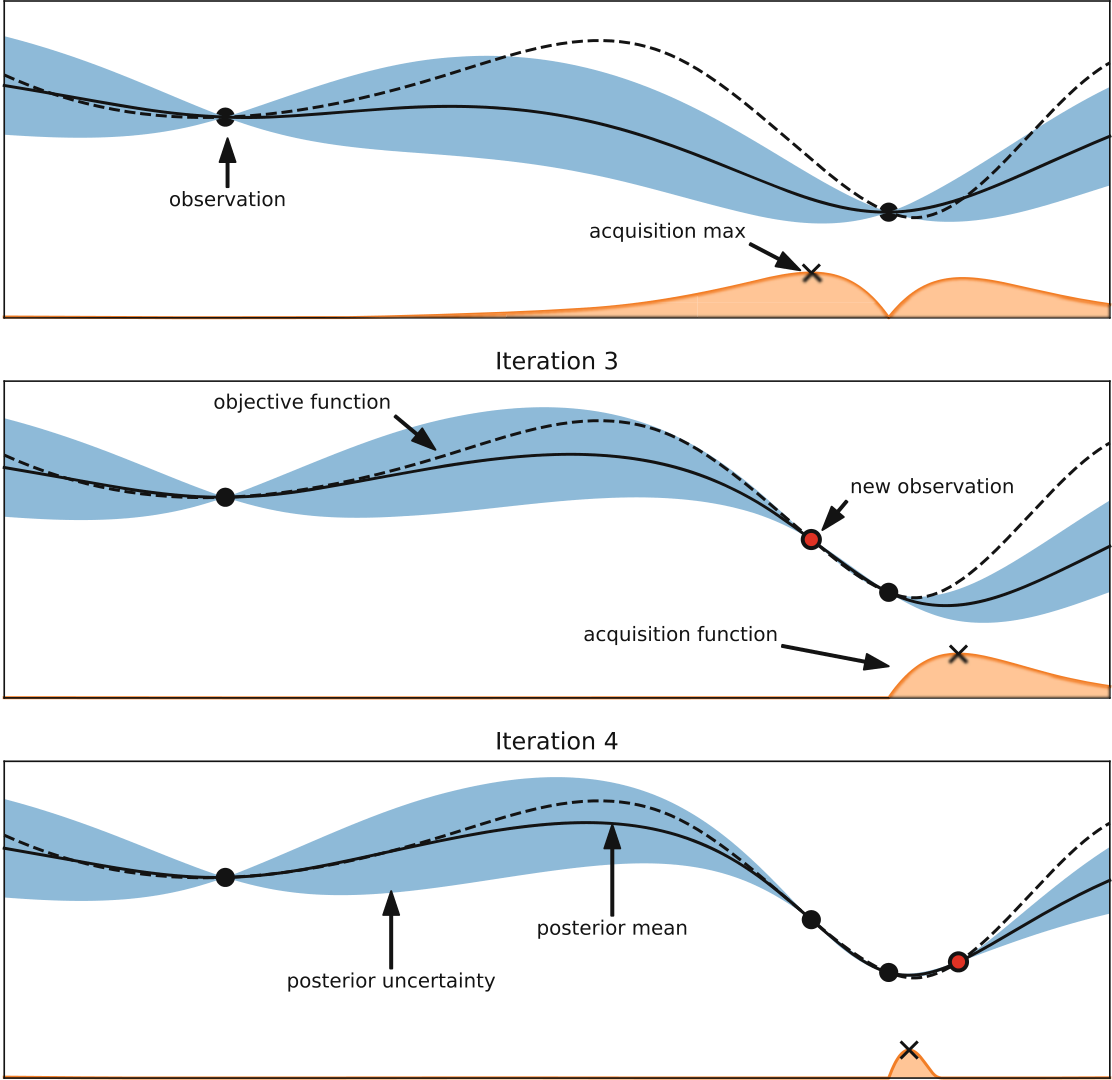
\includegraphics[width=.7\columnwidth]{bayesian.png}
\caption{Máximo error de validación en función de $n_{max}$ y $l_{max}$ para tres diferentes semillas $q_0$. \cite{Feurer2019} }
\label{fig:bayesian}
\end{figure}

 Optimización 1D 

 Comparación

\begin{figure}[h!]
\centering
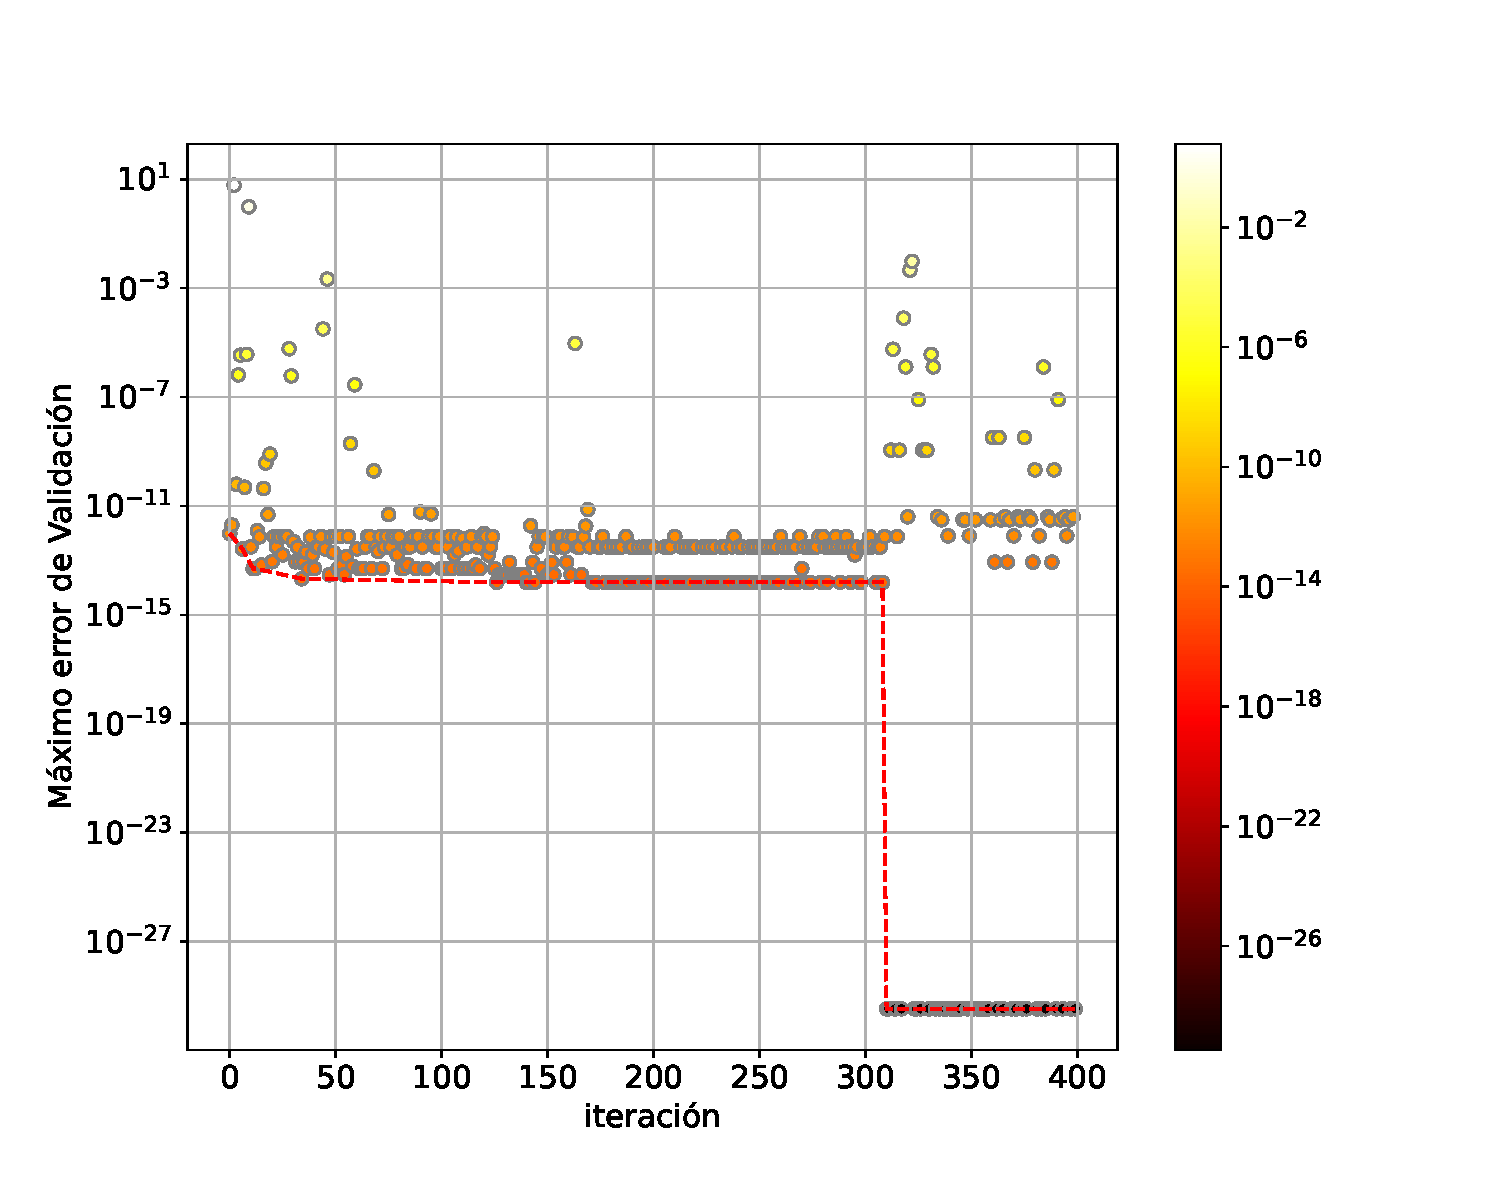
\includegraphics[width=.9\columnwidth, trim={1cm, 1cm, 1cm, 1.1cm}]{opt_1d_value.pdf}
\caption{Máximo error de validación en función de $n_{max}$ y $l_{max}$ para tres diferentes semillas $q_0$. }
\label{fig:optuna_1_value}
\end{figure}

  

\begin{figure}[h!]
\centering
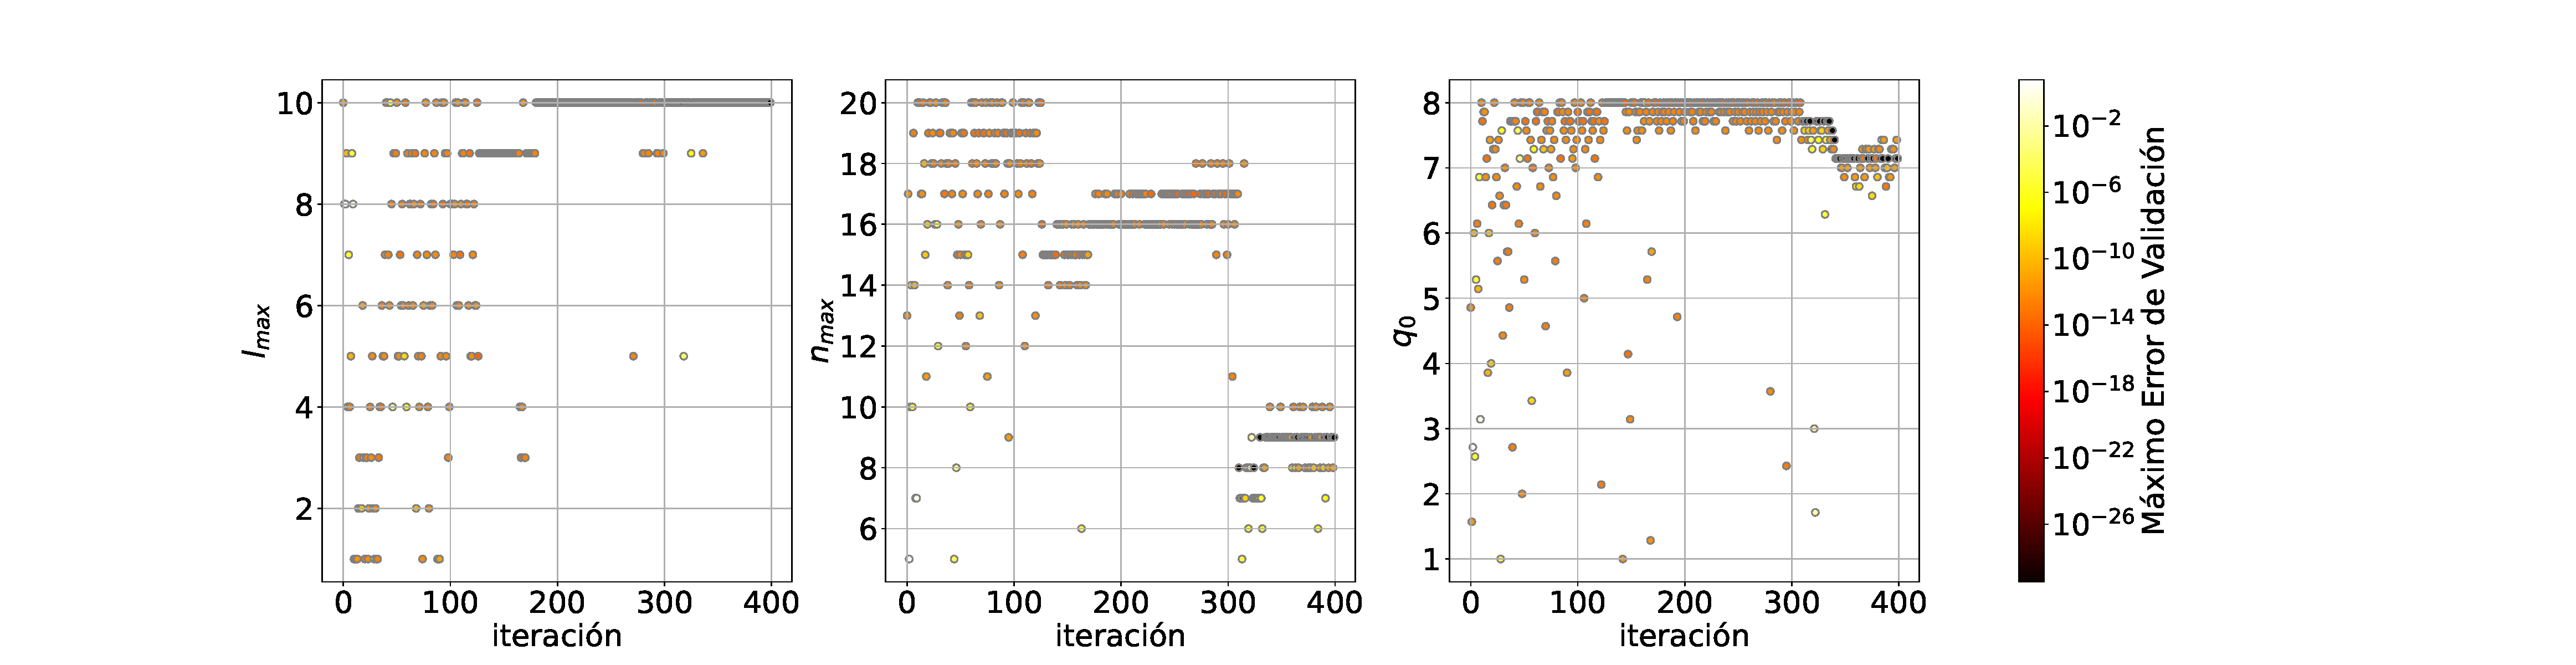
\includegraphics[width=1.05\columnwidth, trim={10cm, 1cm, 10cm, 1.1cm}]{opt_1d_params.pdf}
\caption{Máximo error de validación en función de $n_{max}$ y $l_{max}$ para tres diferentes semillas $q_0$. }
\label{fig:optuna_1_params}
\end{figure}



\subsection{Semilla 1D}



\subsection{Semilla 2D}

\begin{figure}[p!]
\centering
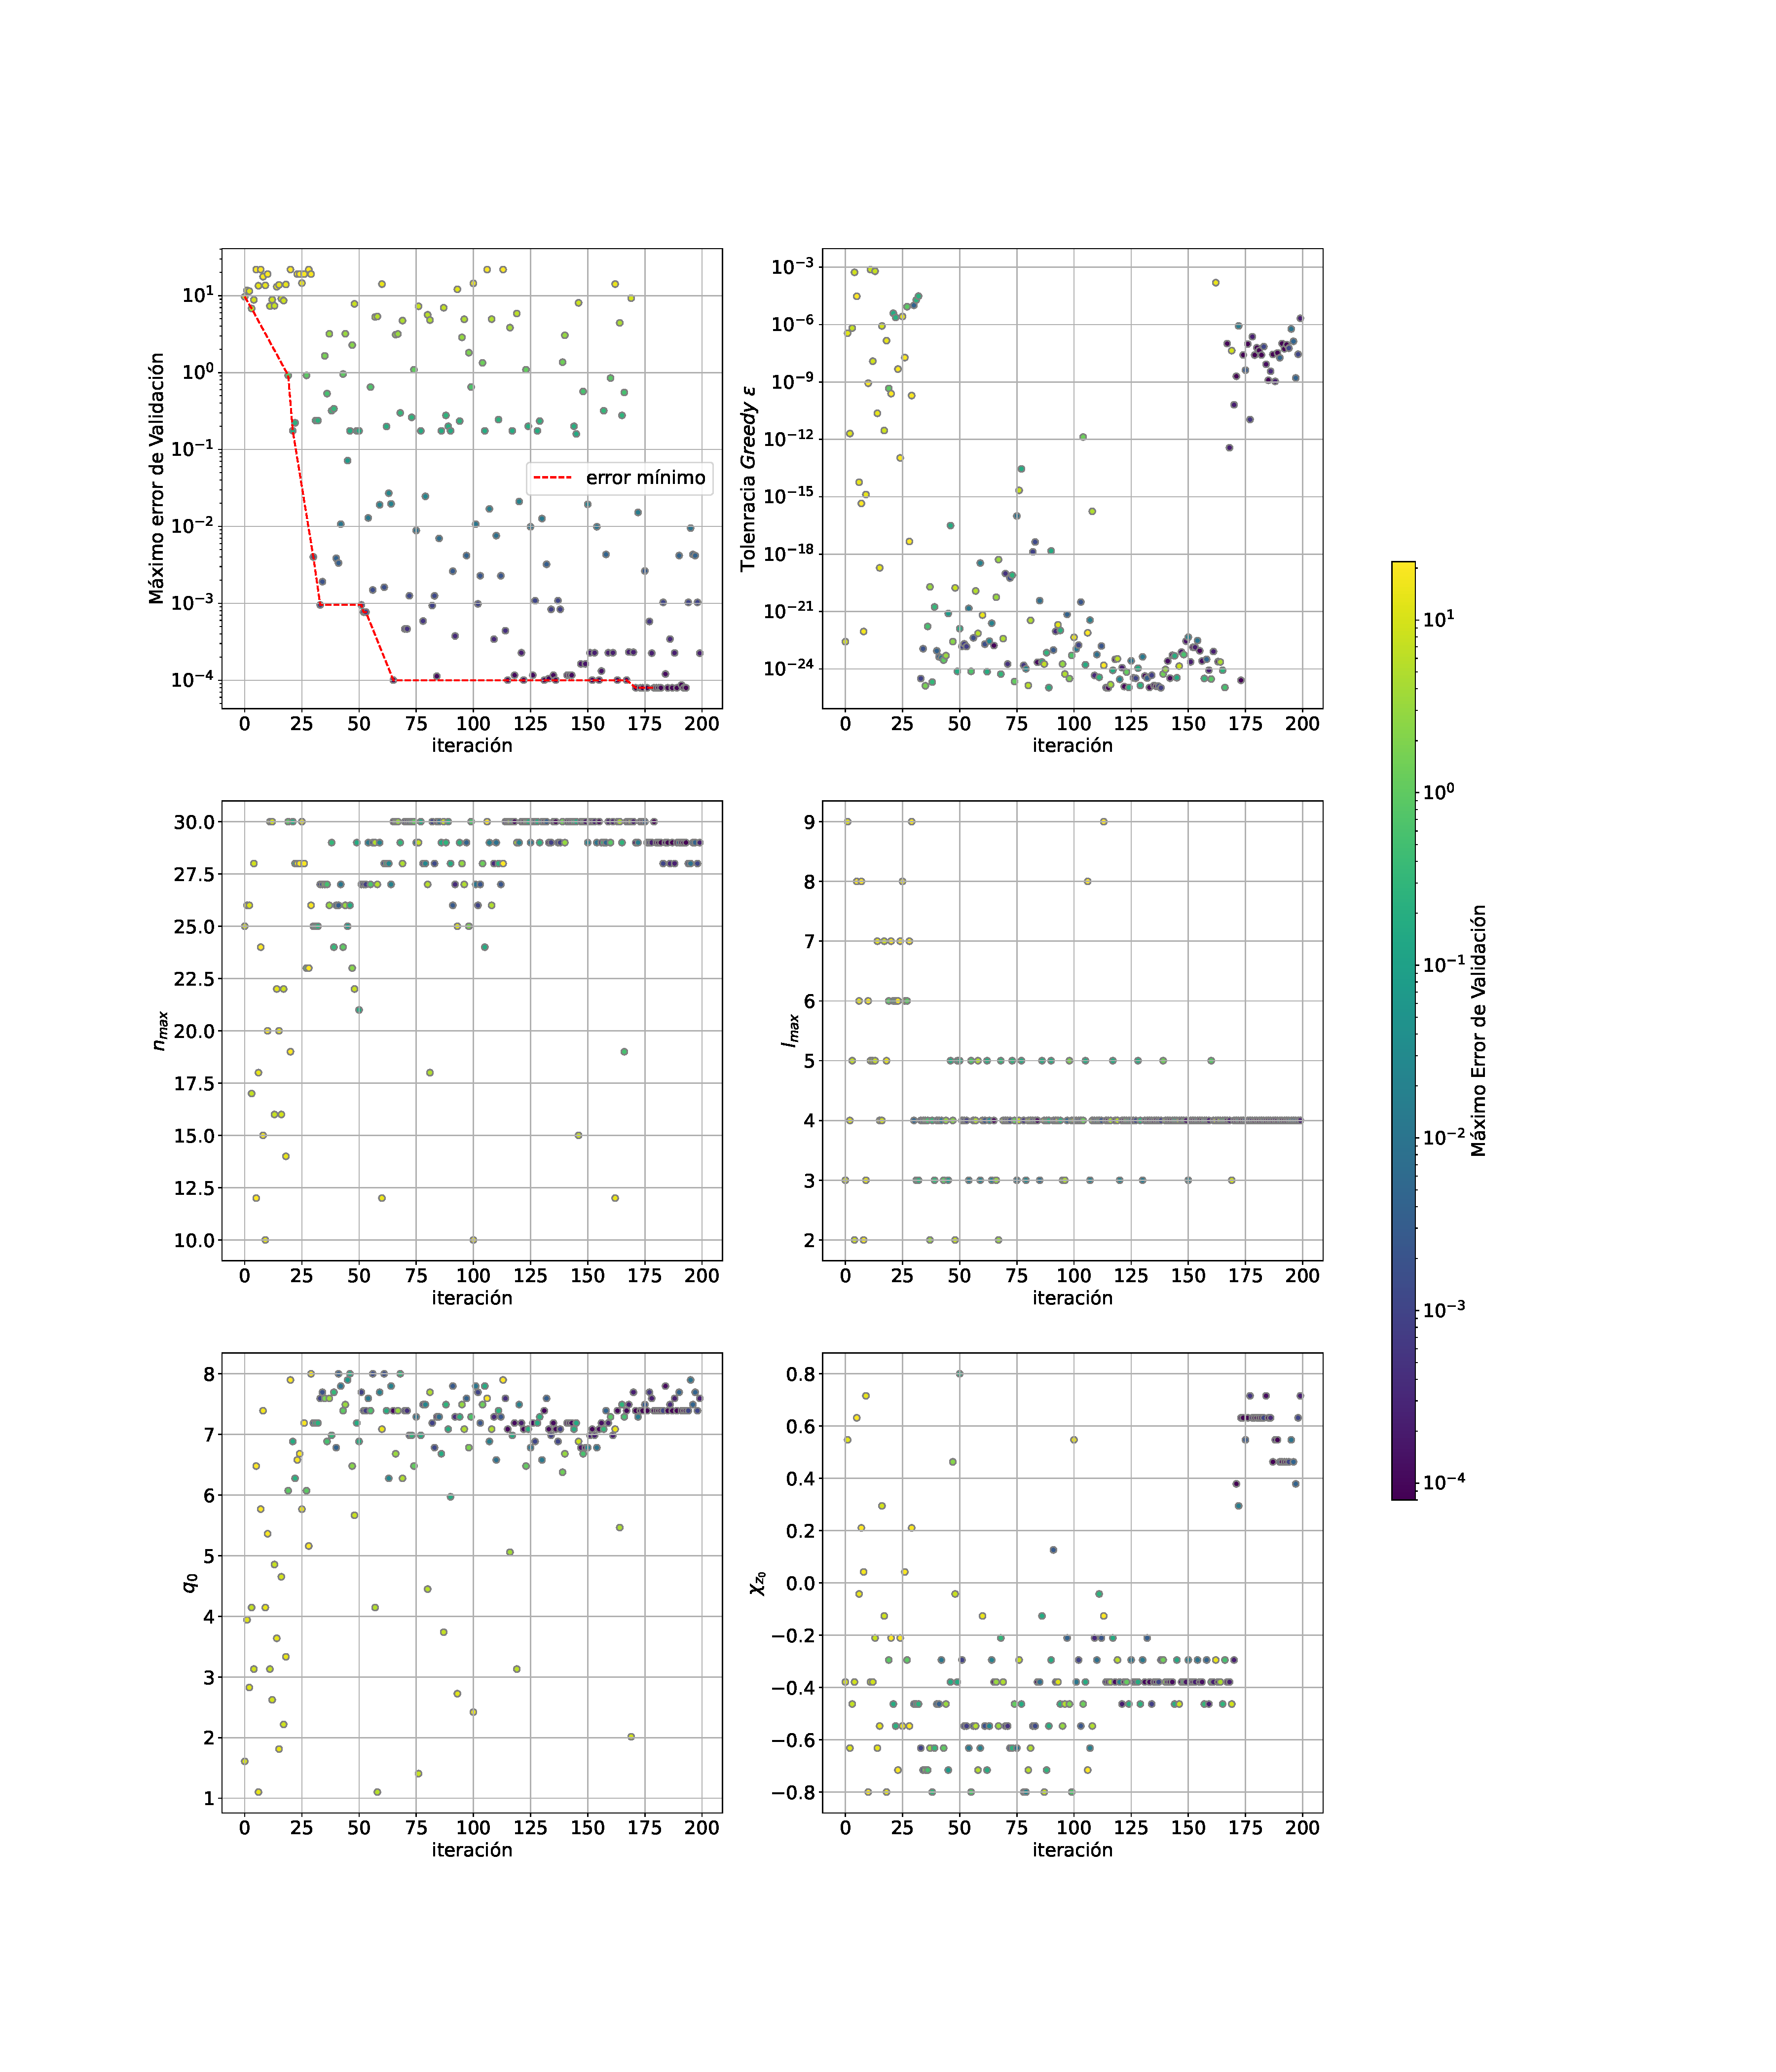
\includegraphics[width=1\columnwidth, trim={6cm, 5cm, 12cm, 5cm}]{Optuna_2D.pdf}
\caption{Máximo error de validación en función de $n_{max}$ y $l_{max}$ para tres diferentes semillas $q_0$. }
\label{fig:optuna_2d}
\end{figure}

2D optimización semilla grid search

 2D optimización semilla optune

 comparación

 Full optimización 2D

 optimización con tiempo

\subsection{Importancia de los Hiperparámetros}